% \documentclass[lettersize,journal]{IEEEtran}

\documentclass[letterpaper,journal]{IEEEtran}
\usepackage{amsmath,amsfonts}
\usepackage{algorithmic}
\usepackage{algorithm}
\usepackage{array}
\usepackage[caption=false,font=normalsize,labelfont=sf,textfont=sf]{subfig}
\usepackage{textcomp}
\usepackage{stfloats}
\usepackage{url}
\usepackage{verbatim}
\usepackage{graphicx}
\usepackage{cite}
\usepackage{multirow}
\hyphenation{op-tical net-works semi-conduc-tor IEEE-Xplore}
% updated with editorial comments 8/9/2021

\begin{document}

\title{A Sample Article Using IEEEtran.cls\\ for IEEE Journals and Transactions}

\author{IEEE Publication Technology,~\IEEEmembership{Staff,~IEEE,}
        % <-this % stops a space
\thanks{This paper was produced by the IEEE Publication Technology Group. They are in Piscataway, NJ.}% <-this % stops a space
\thanks{Manuscript received April 19, 2021; revised August 16, 2021.}}

% The paper headers
\markboth{Journal of IEEE Transactions on Affective Computing, ~Vol.~XX, No.~X, XXXX-2025}%
{Shell \MakeLowercase{\textit{et al.}}: A Sample Article Using IEEEtran.cls for IEEE Journals}

%commentato temporaneamente
%\IEEEpubid{0000--0000/00\$00.00~\copyright~2021 IEEE}
% Remember, if you use this you must call \IEEEpubidadjcol in the second
% column for its text to clear the IEEEpubid mark.

% /////////////////////////////////////////////////////////
% /////////////////////////////////////////////////////////
% /////////////////////////////////////////////////////////


\maketitle
\begin{abstract}
With the global adoption of social networks as primary sources of information and interaction, television has increasingly engaged viewers through social media. This evolution has led to the creation of multimodal corpora, such as EMiT and MultiEMiT.

This paper introduces a new multimodal emotion detection dataset from Italian Twitter posts, annotated according to our particular classification schema. While primarily a resource paper, we also conduct experiments to validate the dataset using transformer models. Our findings show that performance is enhanced by integrating images and text, and is further improved by leveraging the correlations between the diverse annotated labels within the model's prompts.

The datasets utilized consist of Twitter posts related to various Italian TV programs, annotated across five dimensions: emotions, hate speech, irony, target, and the semiotic relationship between text and image in multimodal posts. We developed a dual-model architecture that extracts the final hidden embeddings from both text and image encoders, concatenates these embeddings, and feeds them into a classification head.

Our results, compared to a text-only model, show a 13\% improvement in macro F1 score for emotion recognition on multimodal data when using a concatenation technique. Further tests, incorporating additional information from the other dimensions into the text, resulted in a 15\% improvement over the text-only model, leading to even greater gains in F1 score and precision.

These findings suggest that integrating an image component and prompting additional information significantly enhances the discrimination of emotions in unbalanced and small datasets with noisy data.
\end{abstract}

\begin{IEEEkeywords}
transformers, multimodal, correlations, emotion detection, irony detection, social TV
\end{IEEEkeywords}

\section{Introduction}
\IEEEPARstart{N}{atural} Language Processing (NLP) has emerged as a central discipline within artificial intelligence, significantly influenced by the widespread adoption of social networks. Among its various applications, Sentiment Analysis and Emotion Detection has garnered considerable attention \cite{SOMSA}, playing a crucial role in understanding the emotions and opinions expressed in textual content.

Our research investigates the interaction between text and images within the dynamic landscape of Social TV, where television engages with viewers through social media platforms \cite{SocialTV}. Central to our analysis are two primary datasets. We introduce MultiEMiT, a new multimodal dataset annotated across five distinct levels: emotions, hate speech, irony, target, and the semiotic relationship between text and image in multimodal posts. We also leverage EMiT, an existing corpus annotated only at the target and emotion levels\cite{emit}.

The emotional spectrum used to label these datasets follows the schema proposed by Plutchik, comprising eight primary emotions—joy, sadness, anger, fear, trust, disgust, surprise, and anticipation, with the addition of the categories "love" and "neutral" \cite{Plutchik}.

Additionally, our analysis introduces an annotation level called "semiotic relationship," inspired by Dan Jurafsky's work on determining multimodal intent \cite{MultiM}. This dimension explores the semiotic relationship between text and image, categorizing the relationship into three possible labels: Additive, where text and image mutually enrich each other; Divergent, where text and image differ but combine to create new meaning; and Parallel, where both text and image independently contribute to the same meaning.

The "target" annotation level seeks to determine whether a post's focus is on the transmission itself (container) or its content. 
Upon examining the datasets across these annotation levels, we identified numerous correlations between labels, such as the association between anger and hate, irony and joy, or container and trust.

To enhance the learning process, these correlations were incorporated into the prompts used for training and inference, aiding the model in understanding better the context of the example and improving the results.

Using these annotated datasets on multiple levels, our research aims to uncover the interactions involved in multimodal fusion, highlighting its effects on emotion detection and understanding the context of social television.

The remainder of this paper is structured as follows. Section II reviews related work in Italian sentiment analysis. Section III provides a detailed analysis of the datasets and their annotation schemes. Section IV outlines our experimental design, hypotheses, and methodology. Section V describes the creation of the textual models , which serve as baselines and components for the dual encoder architecture detailed in Section VI. Section VII presents and discusses the results for both emotion and irony detection, analyzing the impact of our correlation prompting technique. Finally, Section VIII concludes the study, summarizing our findings and suggesting directions for future research.


\section{Related Works}

Despite the significant global growth in Sentiment Analysis, most available datasets are in English, reflecting the dominance of English-language content on the web (stata and Brighter?). However, there has been increasing interest in developing corpora to support sentiment analysis in low-resource languages. In the Italian context many resources were created in the last years such as MultiEmotions-It \cite{MultiEmotion}, FEEL-IT \cite{bianchi2021feel} and EMiT\cite{emit}.

\subsection{MultiEmotions-It}
MultiEmotions-It is a dataset created by Rachele Sprugnoli at the Università Cattolica del Sacro Cuore in Milan in 2020. It contains comments on music and advertisement videos posted on YouTube and Facebook, manually annotated on four levels: media-content correlation, polarity, emotions, and sarcasm. Thirty-six students participated in the annotation process, with each student evaluating 90 comments, ensuring that each comment was annotated by two different individuals. For emotion annotation, the dataset utilized Plutchik’s model, which identifies eight basic emotions: joy, sadness, fear, anger, trust, disgust, surprise, and anticipation.

\subsection{FEEL-IT}
Despite differences in sentiment annotation models and data sources, MultiEmotions-It was used in 2021 to test another Italian corpus, FEEL-IT. Created at Bocconi University by Federico Bianchi, Debora Nozza, and Dirk Hovy, FEEL-IT was annotated by Bianchi and Nozza using data from Twitter, collected between August 20 and October 12, 2020, by monitoring trending topics. This approach provided a wide range of posts, covering domains such as health (\#covid19), sports (\#F1), TV shows (\#GFvip), and individuals/politicians (\#DiMaio, \#Suarez). Unlike MultiEmotions-It, FEEL-IT used only four basic emotions: anger, fear, joy, and sadness.

\subsection{EMiT and M.EMO.RAI Project}
The EMiT corpus is part of the M.EMO.RAI project, an artificial intelligence platform developed by the University of Turin's Department of Computer Science in collaboration with the ICT Directorate of Rai \cite{memorai}. The project aims to monitor and analyze viewer emotions, conflicts, debates, and passions on social media related to TV programs.

M.EMO.RAI integrates data from Auditel and Twitter, focusing on spontaneous emotions expressed by the audience. The platform captures various emotions, such as fear, anger, joy, and hate, as well as complex phenomena such as irony. Using an AI engine based on neural networks, the platform analyzes large volumes of social data, combining text analysis of comments with social network analysis of Twitter users involved in discussions about TV broadcasts.

This project enhances traditional TV program ratings, which were primarily based on Auditel data, by incorporating social media sentiment analysis. It aims to provide a comprehensive view of viewer reactions, including specific emotions elicited by broadcasts and the social dynamics within online communities.

M.EMO.RAI is designed to develop an innovative prediction model for viewer appreciation, particularly for new RAI shows. It enables real-time statistical monitoring of viewer reactions, providing quantitative measures of emotional content on social media and indicators of abusive language, hate speech, irony, and sarcasm.

The EMiT corpus, derived from the M.EMO.RAI project, consists of 5,966 posts. These posts were annotated using the same schema as MultiEMiT, using Plutchik's model for emotions and including a target level to indicate whether the posts were directed at the content or the broadcast itself.


\subsection{Evalita 2023}
The EMiT corpus was used in EVALITA 2023 competition, which focused on categorical emotion detection in Italian social media. One notable contribution was from the team extremITA, which developed two systems: extremIT5 and extremITLLaMA.

ExtremIT5 is an Encoder-Decoder model based on IT5, trained by concatenating the task name and an example as input (e.g., “EMiT: Quando ci sarà l’espulsione di Claudia \#ilcollegio [url]”) and producing the sequence of labels as output. In contrast, extremITLLaMA is an instruction-tuned Decoder model built upon the LLaMA foundational models. This model uses a structured prompt in natural language, such as “Which emotions are expressed in this text? You can choose among joy, fear, ...”.


\section{Dataset Analysis}
This study primarily focuses on the MultiEMiT corpus, a multimodal dataset of Twitter posts generated by interactions with TV programs. Specifically, MultiEMiT includes data from the shows PropagandaLive and Pechino Express \cite{propagandalive,pechinoexpress}. In addition to MultiEMiT, we also utilize the EMiT (Emotions in Italian) corpus \cite{emit}, which contains posts from a wider range of Italian TV shows such as Festival di Sanremo, Don Matteo, and Il Collegio. However, in this work, EMiT is employed exclusively as a supplementary resource to fine-tune the emotion detection models, thereby enhancing their robustness when applied to the MultiEMiT dataset.

\subsection{Context of the Data: PropagandaLive and Pechino Express}

Before proceeding with the steps for creating the MultiEMiT corpus, it is necessary to provide context for the initial datasets.

PropagandaLive is a satirical talk show that has been airing on LA7 since 2017, hosted by Diego Bianchi. The episode chosen to form the initial dataset aired on November 19, 2021. During this period, many migrants were blocked at the border between Poland and Belarus, provoking a strong emotional response across Europe. Diego Bianchi, accompanied by actress and activist Kasia Smutniak and director Pierfrancesco Citriniti, decided to travel to the border to report and show what was happening in the area.

The Pechino Express data originated from the first episode of the eighth edition of the show. Pechino Express is an Italian reality and adventure television program. The format of the show consists of a race between pairs of acquaintances, both famous and non-famous, who compete along a route crossing multiple countries to reach a designated destination in a multi-day stage journey.

\subsection{Labeling}
MultiEMiT was annotated on five distinct levels: Emotions, Irony, Hate, Target, and Image-Text Relation.
It was labeled by three different annotators; for all of them, it was the first time performing a labeling task, but all the annotators had a background in either computer science or linguistics. The gold standard was established when at least two out of three annotators agreed on the label.

A single post can express multiple emotions simultaneously. According to Plutchik’s emotion schema, combinations of emotions can form new emotions \cite{Plutchik}. For instance:
Trust + Joy = Love or
Anger + Surprise = Outrage.
This combinatory approach helps in capturing the nuanced emotional states expressed in the posts. An illustrative schema (Figure \ref{fig:dyad}) provides further details on these combinations.
\begin{figure}
  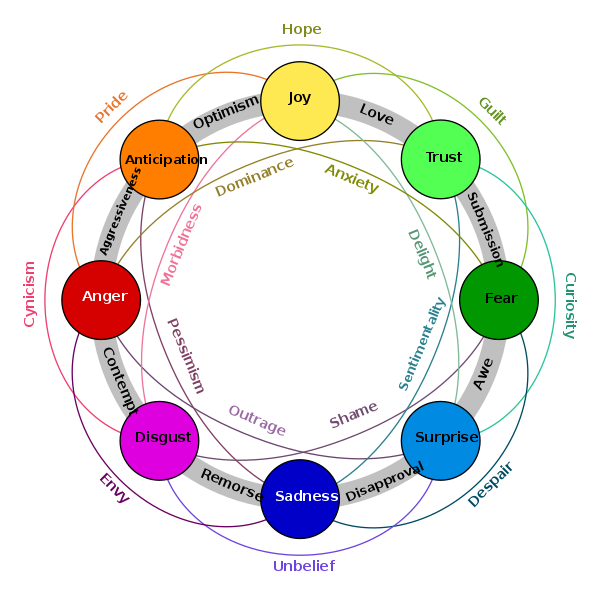
\includegraphics[width=\linewidth]{imgs/Plutchik_Dyads.svg.png}
  \caption{Plutchik Dyads of emotions}
  \label{fig:dyad}
\end{figure}

The target level aims to determine whether the post is directed towards the topic of the TV program or the transmission itself. It is possible for a single post to carry both labels. For instance, a post might comment on the quality of the broadcast (direction) while also discussing specific content within the show.

Based on Jurafsky’s studies \cite{MultiM}, the relation between text and image in multimodal posts can be classified into three categories: Additive, where the information from the text and image mutually enrich each other; Divergent, where the text and image provide differing information, but their combination yields a new meaning; and Parallel, where both the text and image independently contribute to the same meaning. Examples can be seen in the image shown in Figure \ref{fig:relations}.

\begin{figure}
  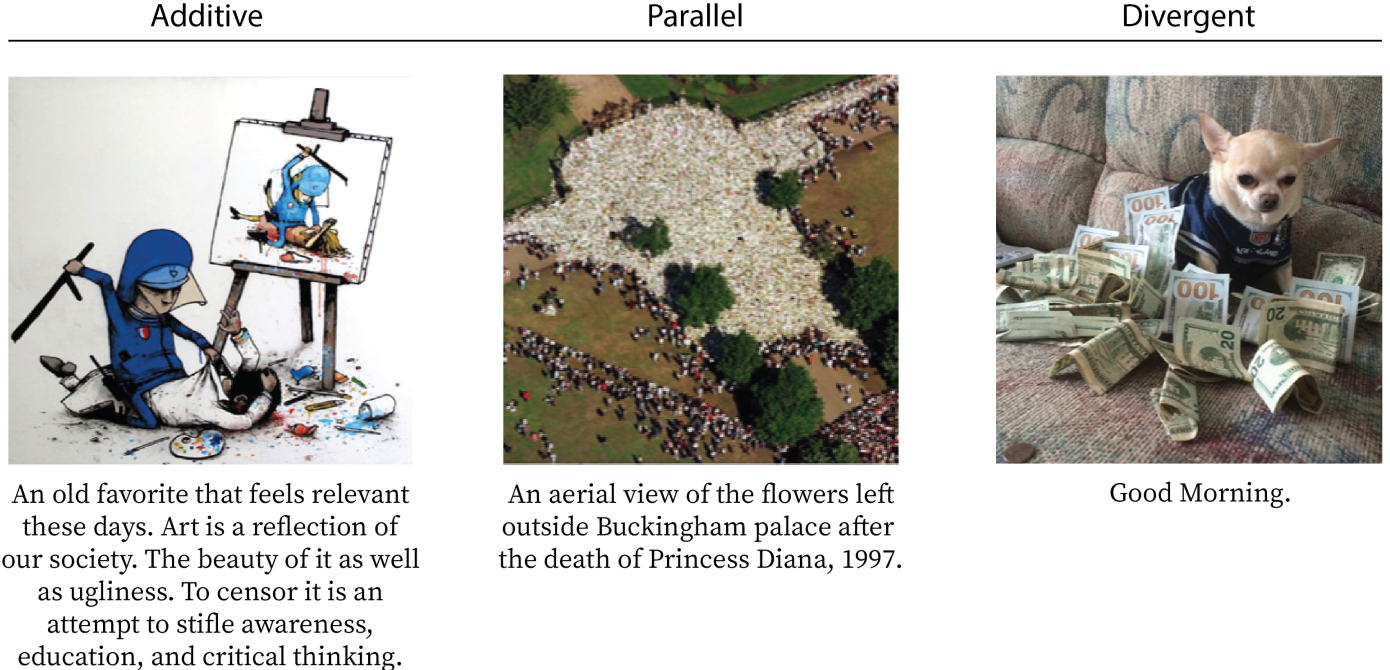
\includegraphics[width=\linewidth]{imgs/Additive_divergent_parallel.png}
  \caption{Examples of semiotic relationship}
  \label{fig:relations}
\end{figure}

Hate and irony levels are binary features indicating the presence of hate speech or ironic content in the posts.

\subsection{Labels Distribution}
After creating the gold standard, where a label was kept if at least two out of three annotators agreed, we obtained two datasets: a textual dataset, without an image component, consisting of 2,909 posts, and a multimodal dataset consisting of 645 posts. The distribution of labels in these datasets is shown in Table \ref{table:2}.


% Table 2 - Distribution of MultiEMiT multimodal data
\begin{table}[!t]
\caption{Distribution of MultiEMiT.}
\label{table:2}
\centering
\begin{tabular}{llcc}
\textbf{Level}        & \textbf{Label} & \textbf{Textual (2,909 posts)} & \textbf{Multimodal (645 posts)} \\ \hline
\textbf{Emotions}     & Anger          & 163                            & 34                              \\
                      & Anticipation   & 201                            & 61                              \\
                      & Disgust        & 410                            & 78                              \\
                      & Fear           & 55                             & 4                               \\
                      & Joy            & 552                            & 168                             \\
                      & Love           & 340                            & 50                              \\
                      & Neutral        & 763                            & 255                             \\
                      & Sadness        & 255                            & 25                              \\
                      & Surprise       & 486                            & 82                              \\
                      & Trust          & 613                            & 214                             \\ \hline
\textbf{Hate}         & Hate           & 53                             & 7                               \\ \hline
\textbf{Irony}        & Irony          & 509 (481)                      & 121 (109)                       \\
                      & Sarcasm        & 41 (13)                        & 20 (8)                          \\
                      & Non-ironic       & 2387                           & 516                             \\ \hline
\textbf{Target}       & Content        & 1065                           & 192                             \\
                      & Container      & 1074                           & 388                             \\
                      & Both           & 73                             & 7                               \\
                      & None           & 697                            & 58                              \\ \hline
\textbf{Relationship} & Additive       & //                             & 389                             \\
                      & Divergent      & //                             & 158                             \\
                      & Parallel       & //                             & 100                             \\ \hline
\end{tabular}
\end{table}

Due to the numerous labels and the various ways to interpret the same sentence, many potential labels were omitted in the gold standard because it required at least two out of three annotators to agree on the same label. For example, given the post depicted in Figure \ref{fig:interpretation_of_posts}, each annotator had a different interpretation: annotator 1 labeled it as "Anger and Disgust" towards Europe, the second annotator labeled it as "Sadness and Surprise" indicating disapproval, and the third annotator labeled it as "Disgust and Fear" interpreting it as shame of being European. In the process of creating the gold standard, only the label "Disgust" was retained, while all other interpretations were discarded.

\begin{figure}[!t]
\centering

\includegraphics[width=2.5in]{imgs/interpretation_of_posts.png}
\caption{Example of Twitter post with multiple interpretations}
\label{fig:interpretation_of_posts}
\end{figure}

\subsection{Labels correlations}
As previously mentioned, the presence of numerous labels within the same dataset prompted us to investigate their correlations. Figures \ref{fig:emotions_correlations}, \ref{fig:relations_correlations}, and \ref{fig:irony_correlations} illustrate the Pearson correlation between the primary annotation levels.
\begin{figure}[!t]
\centering
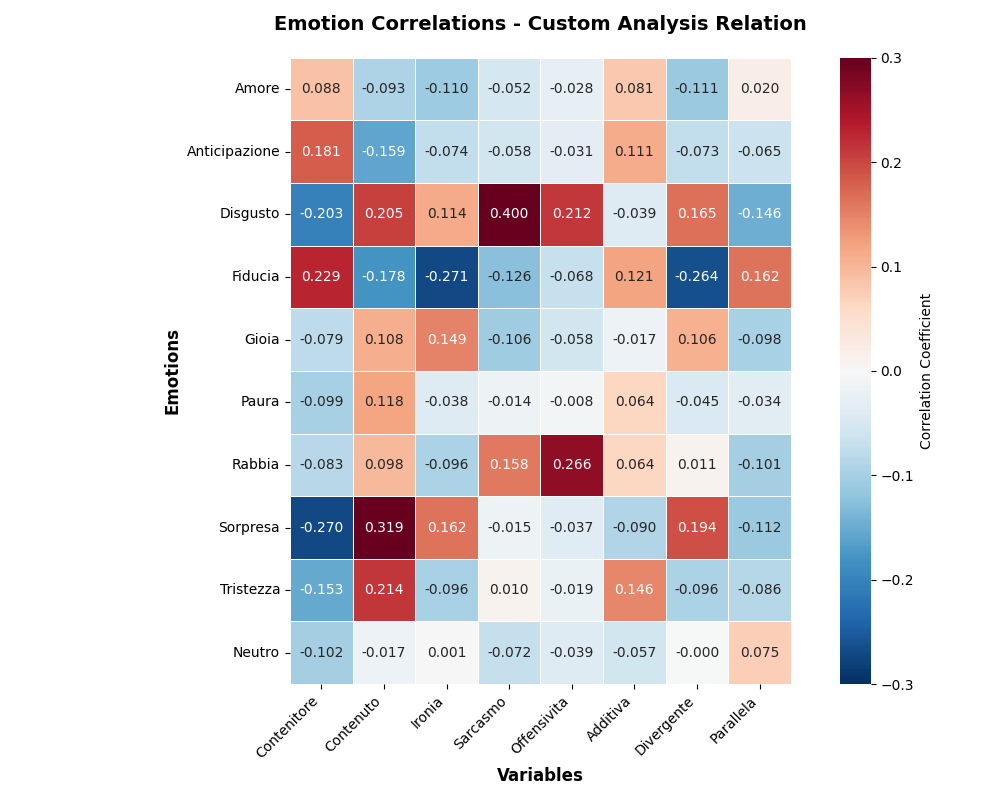
\includegraphics[width=2.5in]{imgs/emotion_correlations_EM_PROS.png}
\caption{Pearson correlation between Emotions and other labels}
\label{fig:emotions_correlations}
\end{figure}

\begin{figure}[!t]
\centering
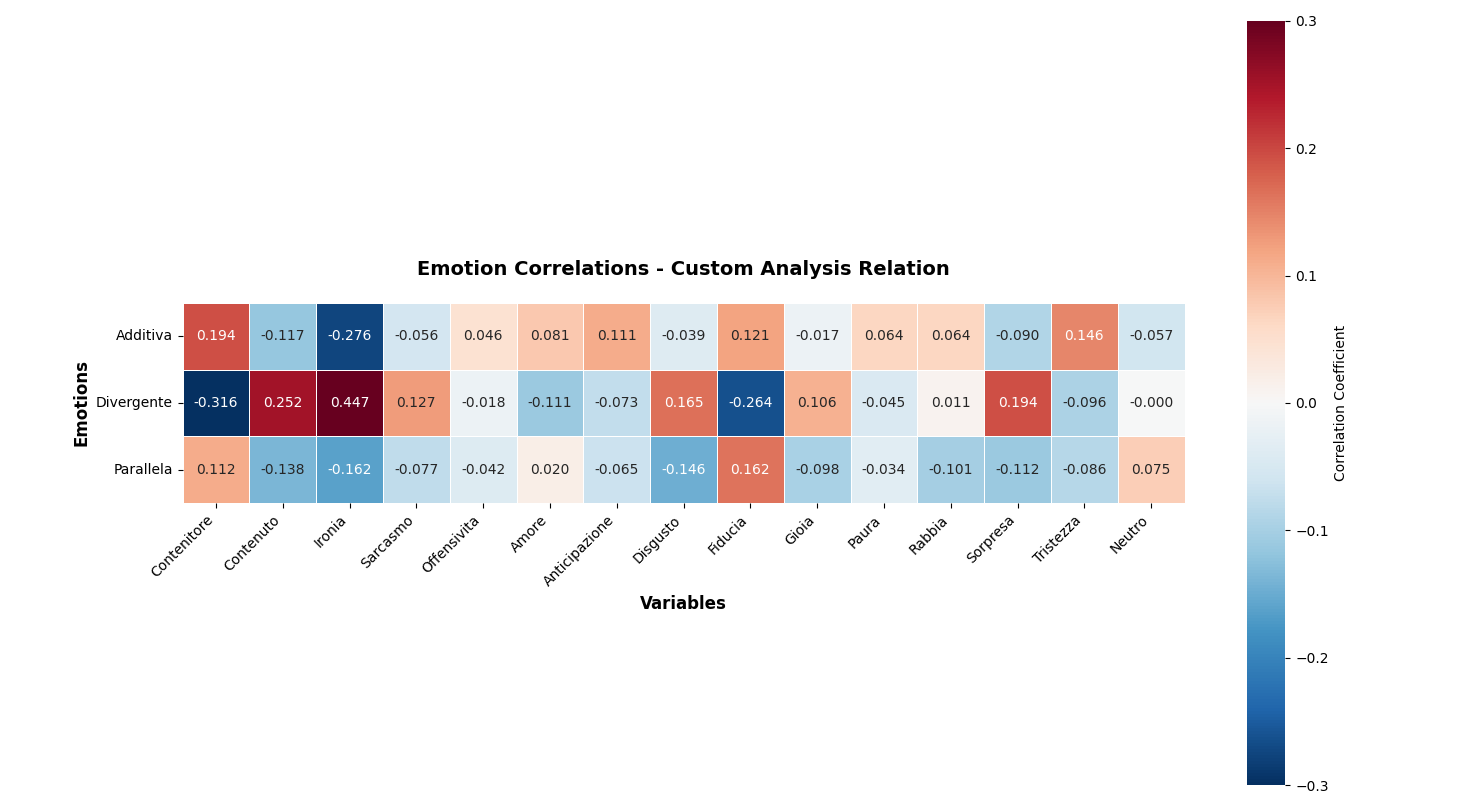
\includegraphics[width=\linewidth]{imgs/relation_correlations_EM_PROS.png}
\caption{Pearson correlation between Semiotic Relations and other labels.}
\label{fig:relations_correlations}
\end{figure}

\begin{figure}[!t]
\centering
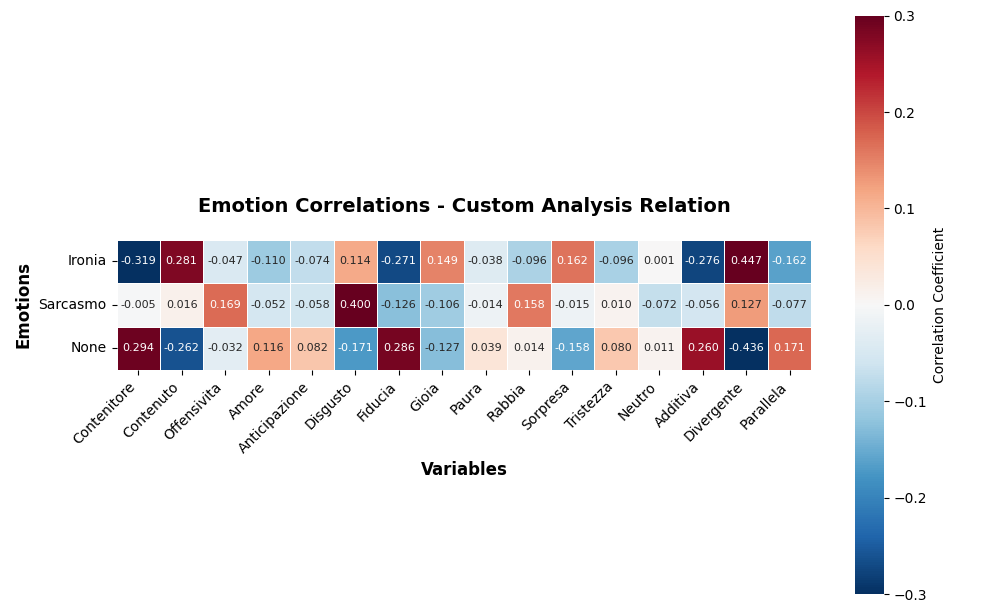
\includegraphics[width=2.5in]{imgs/irony_correlations.png}
\caption{Pearson correlation between Irony and other labels}
\label{fig:irony_correlations}
\end{figure}

In Figure \ref{fig:emotions_correlations}, we observe the correlations between Emotions and all other annotation levels. It is evident that Irony and the Divergent relation share a similar pattern of correlations with Emotions. Typically, posts with a Divergent relationship between text and image are related to memes or humorous content. Additionally, we observe that Offensiveness is closely associated with emotions like Disgust and Anger. In contrast, posts related to Direction (container) are more commonly linked to Trust and Anticipation, whereas those focusing on the Topic (content) of the program are often connected to Surprise, Disgust, and Sadness.

Figure \ref{fig:relations_correlations} provides a focused look at the correlations between the three semiotic relationships and the other labels. This view confirms the strong connection between the Divergent relation and non-literal content, showing its strongest positive correlations with Sarcasm and Irony. It also co-occurs with emotions like Anger and Disgust, while being negatively correlated with Trust and the Direction (container) of the post. In contrast, the Additive relation shows only mild positive correlations, such as with Trust and Anticipation. The Parallel relation is most notable for its lack of strong correlations, with its most significant associations being weakly negative with Direction and Disgust.

On the other hand, Figure \ref{fig:irony_correlations} focuses on the correlations between Irony and the other levels. This figure highlights that Irony and the Divergent relation exhibit the strongest correlation among the dimensions analyzed. Specifically, Irony is more frequently found in posts discussing the Topic, and is often associated with emotions such as Disgust and Joy, while showing a negative correlation with Direction, Additive relation, and Trust. 

These observed correlations motivated us to integrate them directly into the text, as demonstrated in Table \ref{table:prompting}, to enhance the model's ability to classify complex, multimodal posts more accurately.

% Table 3 - Example of correlations prompted
\begin{table*}[htb!]
\begin{center}
{\footnotesize
\begin{tabular}{l|l}
\hline
& \textbf{Italian text} \\
\hline
\textit{Original} & ma soleil é con sua nonna? \\
\textit{Prompted} & il seguente testo contiene ironia e offensività riguarda contenitore: ma soleil é con sua nonna? \\
\hline
& \textbf{English text} \\
\hline
\textit{Original} & is soleil with her grandma? \\
\textit{Prompted} & the following text contains irony and offensivity regards the direction: is soleil with her grandma? \\
\hline
\end{tabular}
}
\end{center}
\setlength{\belowcaptionskip}{-0.1cm}
\caption{Example of correlations prompted.}
\label{table:prompting}
\end{table*}

This method of prompting provides the model with indicators regarding the various levels relative to the classification one, improving its capability to accurately classify posts.


\section{Experimental Design}
The primary objective of our experimental procedure is to systematically evaluate the classification of emotions and irony in complex, multimodal social media posts. The core challenges of this task stem from the nature of the data: the datasets are small, inherently noisy, unbalanced, and require models to interpret the intricate and often non-literal relationships between text and images. Furthermore, the classification is not only multiclass but also multi-label, as a single post can simultaneously express multiple emotions.

Our experiments are designed to address two primary hypotheses:
\begin{enumerate}
    \item That a multimodal model, which can process both text and images, will significantly outperform a text-only model on this dataset.
    \item That explicitly providing the model with contextual information about \textit{other} annotation layers—our "correlation prompting" technique—will further improve the classification performance for both text-only and multimodal models.
\end{enumerate}

We tested these hypoteheses thoutgh a structured three-phase experimental approach:

\subsection{Text-Only Model}
First, we establish strong textual baselines. We leverage pre-trained Italian BERT models—specifically, the \texttt{feel-it-italian-emotion} model for emotion classification \cite{bianchi2021feel} and \texttt{UmBERTo} for irony detection \cite{musixmatch-2020-umberto}. We finetune these models on our textual data from the MultiEMiT and EMiT corpora \cite{emit}. This phase evaluates the performance of text-only models and, critically, provides the first test of our correlation prompting hypothesis by comparing models trained with and without this additional textual information. These finetuned models also serve as the text-encoder component for Phase 2.

\subsection{Multimodal Model}
In the second phase, we develop our dual-encoder multimodal architecture. This model is composed of:
\begin{itemize}
    \item \textbf{A Text Encoder:} The best-performing finetuned BERT model from Phase 1.
    \item \textbf{An Image Encoder:} A pre-trained Vision Transformer (ViT) \cite{dosovitskiy2021vit}.
\end{itemize}
The final hidden embeddings from both encoders are concatenated and passed to a classification head. We then train this architecture on the multimodal subset of the MultiEMiT dataset. We run these experiments for emotion, irony, and text-image relation detection, again comparing the performance of models with and without correlation prompting to quantify the combined benefit of the visual modality and our prompting technique.

\subsection{Comparative Analysis with Pixtral LLM}
Finally, we benchmark our specialized, finetuned multimodal model against Pixtral, a state-of-the-art multimodal Large Language Model (LLM). The objective here is to determine if a general-purpose LLM, given sophisticated prompting, can match or exceed the performance of a smaller, domain-specific finetuned model on such a noisy and unbalanced dataset. We test this using zero-shot and three-shot prompting strategies and explicitly investigate whether augmenting the LLM's prompts with our correlation information can bridge the performance gap.


\section{Creation of the Textual Model}
In this section, we describe the creation and validation of our textual models. The primary objective of this phase was to assess the consistency and learnability of our newly annotated dataset. To establish robust baselines, we leveraged existing Italian resources, specifically utilizing FEEL-IT \cite{bianchi2021feel} for emotion recognition and IRONITA \cite{ironita2018} for irony detection. By fine-tuning models on the textual data, we verified that the annotations were robust enough to train a classifier effectively. Once validated, these models served as the foundation for our subsequent experiments: they provided the text-only benchmark for the multimodal dataset and acted as the pre-trained text encoder for our dual-model architecture.

\subsection{Pretrained Models: FEEL-IT and UmBERTo}
To build an effective architecture, we required text encoders already adapted to Italian sentiment analysis. For emotion classification, rather than starting from a generic BERT model, we utilized \texttt{feel-it-italian-emotion} \cite{bianchi2021feel}, a BERT-based model pre-trained on the FEEL-IT corpus. Designed specifically for Italian emotion recognition, it provided a strong initialization for our tasks. For irony and relation detection, we employed \texttt{UmBERTo} \cite{musixmatch-2020-umberto}, a state-of-the-art Italian language model trained with Whole Word Masking, which we further fine-tuned on the IRONITA dataset \cite{ironita2018}.

\subsection{Emotion Detection Model}
We tested many different label encodings to find the most effective representation. Following Plutchik’s theory \cite{Plutchik}, we acknowledged that multiple emotions often coexist in a single post.

Initial experiments treating every unique combination of emotions as a distinct class (resulting in 27 labels) proved too sparse, yielding poor performance. Reducing this to 20 broader labels improved results slightly, but significant gains were only observed when simplifying to the six primary emotions (joy, sadness, disgust, fear, surprise, anger) plus \textit{Neutral}.

To address class imbalance—specifically the scarcity of \textit{fear} samples—we merged \textit{fear} into \textit{sadness} and introduced \textit{love} as a distinct primary category. While this improved the F1 score to nearly 0.40, the single-label approach required aggressive oversampling, leading to overfitting. Consequently, we transitioned to a \textbf{multi-label classification framework} using a one-hot encoding scheme. This allowed the model to predict the presence of each emotion independently. Using a probability threshold of 0.4, this configuration achieved a macro F1 score of 0.46 on the MultiEMiT test set (Table \ref{table:emotion}).

We further enhanced performance by integrating correlation information directly into the text prompts. We compared two initialization strategies:
\begin{enumerate}
    \item \textbf{Standard Initialization:} Fine-tuning the original \textit{feel-it} model with correlation-augmented text, which improved the F1 score to 0.54.
    \item \textbf{General Model Initialization:} We also evaluated a "General Model" trained and tested on the combined EMiT and MultiEMiT datasets, which provided a baseline F1 of 0.49. When this robust general model was fine-tuned with correlation prompts, it achieved our best textual performance with a Macro F1 of 0.59 and an accuracy of 0.41.
\end{enumerate}

The solid performance on the textual test set confirms the consistency of the dataset. Consequently, this model was selected to serve as the text encoder for the multimodal architecture.

% Performance tables with proper formatting
\begin{table*}[htb!]
\begin{center}
{\footnotesize
\begin{tabular}{l|c|c}
\hline
\textbf{Model Name} & \textbf{Macro F1} & \textbf{Accuracy} \\
\hline
Feel-IT Finetuned (MultiEMiT test) & 0.46 & 0.32 \\
Feel-IT Finetuned w/ Correlations (MultiEMiT test) & 0.54 & 0.38 \\
Base General Model (Combined test) & 0.49 & 0.32 \\
Base General Model w/ Correlations & \textbf{0.59} & \textbf{0.41} \\
extremIT5 & 0.60 & -- \\
extremITLLaMA & 0.50 & -- \\
\hline
\end{tabular}
}
\end{center}
\setlength{\belowcaptionskip}{-0.1cm}
\caption{Emotion Detection Model Performance (Textual).}
\label{table:emotion}
\end{table*}

Figure \ref{fig:evo} depicts a comprehensive graph illustrating the model's progression across all tests.
\begin{figure}[t]
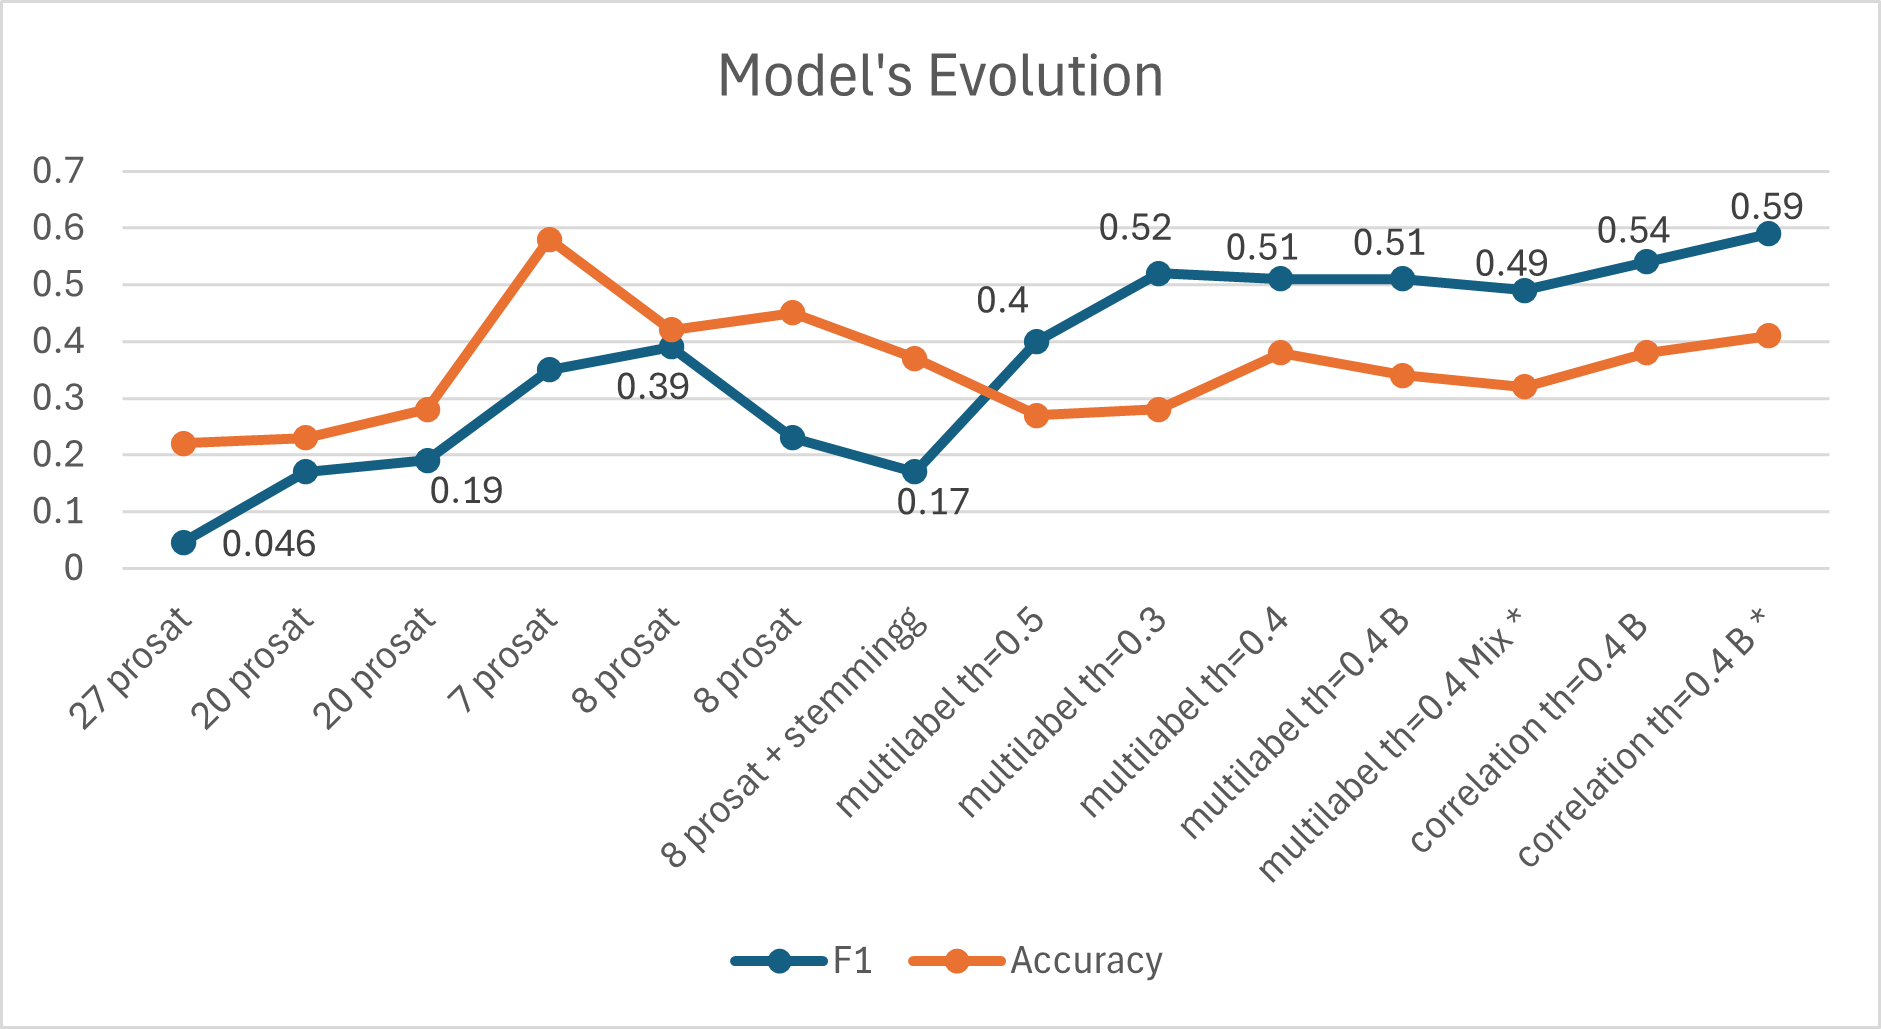
\includegraphics[width=\linewidth]{imgs/model_evo.png}
\caption{Evolution of the emotion detection model}
\label{fig:evo}
\end{figure}

\subsection{Irony Detection Model}
Our irony detection model was developed by fine-tuning the UmBERTo model on the IRONITA dataset \cite{ironita2018} and subsequently on our internal data. We evaluated the impact of context by training models with and without correlation prompts. As shown in Table \ref{table:irony}, the inclusion of correlation data significantly boosted performance, raising the Macro F1 score from 0.44 to 0.52.

\begin{table}[htb!]
\begin{center}
{\footnotesize
\begin{tabular}{l|c|c}
\hline
\textbf{Model Name} & \textbf{Macro F1 Score} & \textbf{Accuracy} \\
\hline
Pre-trained IRONITA & 0.39 & 0.82 \\
Textual Model without Correlations & 0.44 & 0.82 \\
Textual Model with Correlations & 0.52 & 0.84 \\
\hline
\end{tabular}
}
\end{center}
\setlength{\belowcaptionskip}{-0.1cm}
\caption{Irony Detection Model Performance.}
\label{table:irony}
\end{table}

\subsection{Image-Text Relation Model}

We also evaluated the impact of correlations on image-text relation detection. Although extracting relationships from textual components alone might seem challenging, this method helps identify words associated with each class, improving the encodings for the final architecture. Using the same UmBERTo model as for irony detection \cite{musixmatch-2020-umberto}, we created models with and without correlations. The F1 score improved from 0.66 to 0.70, and accuracy increased from 0.68 to 0.72. The performance metrics for the image-text relation detection models are summarized in Table \ref{table:relation}.

\begin{table}[htb!]
\begin{center}
{\footnotesize
\begin{tabular}{l|c|c}
\hline
\textbf{Model Name} & \textbf{Macro F1 Score} & \textbf{Accuracy} \\
\hline
Textual Model without Correlations & 0.66 & 0.68 \\
Textual Model with Correlations & 0.70 & 0.72 \\
\hline
\end{tabular}
}
\end{center}
\setlength{\belowcaptionskip}{-0.1cm}
\caption{Image-Text Relation Detection Performance.}
\label{table:relation}
\end{table}


\section{Multimodal Model Architecture}
In this section, we describe the dual model architecture used for emotion and irony detection.

Our proposed model comprises two main components: a text encoder and an image encoder, both based on transformer architectures. These architectures have demonstrated superior performance in various natural language processing (NLP) and computer vision tasks.

The text encoder utilises a pre-trained BERT model \cite{devlin2019bert} to extract contextual embeddings from the textual data. BERT's bidirectional attention mechanism enables it to understand the context of a word by looking at both its preceding and following words, making it well suited for sentiment and emotion analysis. Initially, we tested with a standard Italian BERT model trained for masked language modeling (MLM). Later, a BERT model was fine-tuned specifically for emotion classification using the textual data, which significantly improved the encoder's performance.

The image encoder is based on a pre-trained Vision Transformer (ViT) model \cite{dosovitskiy2021vit}, which processes images by dividing them into patches and applying transformer layers to capture the spatial relationships between these patches. After evaluating several image classification models, we found that Google's ViT model delivered the best performance, making it the optimal choice for our image encoder.

The outputs of the text and image encoders are concatenated to create a joint representation of the multimodal input. This concatenated embedding is then passed through a fully connected layer, which acts as the classifier head. We tested various classifier heads from Scikit-Learn, selecting the one that yielded the best results for the final model. A normalization layer is applied afterward to ensure the stability and performance of the classification process.

In the Results section, we compare the performance of the multimodal model to that of a text-only model applied to the same multimodal dataset. This comparison underscores the benefits of incorporating visual data alongside textual data in tasks involving emotion and irony detection. The overall architecture of the model is illustrated in Figure \ref{fig:architecture}.

\begin{figure}[t]
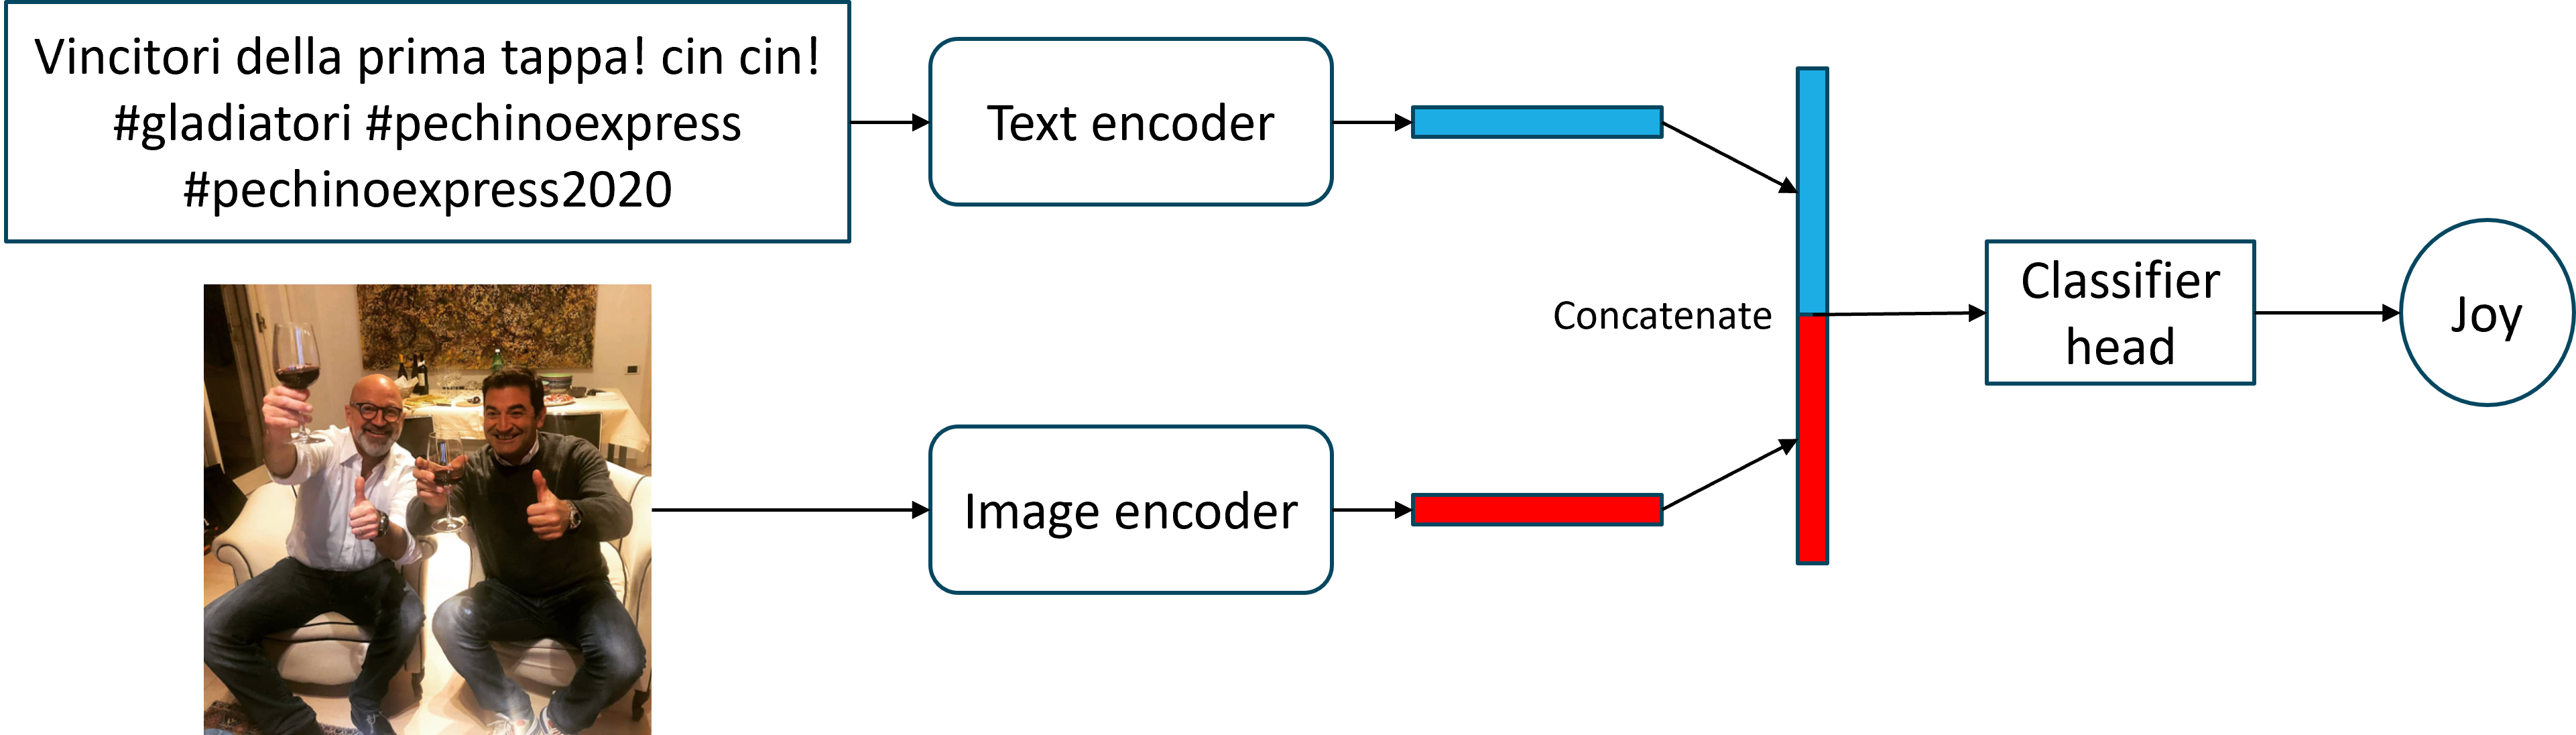
\includegraphics[width=\linewidth]{imgs/model_architecture.png}
\caption{Dual Model Architecture for Multimodal Emotion and Irony Detection}
\label{fig:architecture}
\end{figure}


\section{Multimodal Model Results}

In this chapter, we analyze the performance of our models on multimodal emotion and irony detection tasks. The results demonstrate the effectiveness of incorporating correlation information and the advantages of using multimodal approaches.

\subsection{Emotions}

Table \ref{tb:emotion_multi} presents the performance of our multimodal emotion detection models. Without correlations, the model achieved a precision of 0.39 and an F1 score of 0.43. The text-only model had a significantly lower F1 score of 0.30, highlighting the benefit of using multimodal data. When correlations were included, the model's performance improved across all metrics, with precision increasing to 0.43 and the F1 score to 0.45. The text-only model with correlations also showed improvement, achieving an F1 score of 0.37. The addition of correlation information led us to examine the improvements in emotion detection within each subset of the multimodal data. We found that the micro F1 scores increased from 0.47 to 0.54 for the Additive subset, from 0.52 to 0.60 for the Parallel subset, and from 0.38 to 0.42 for the Divergent subset, which correspond to specific text-image relations.

These results highlight the clear advantage of using multimodal data for emotion detection. The incorporation of correlation information further enhances the model's performance, suggesting that understanding the relationships between different modalities and contextual information is crucial for accurate sentiment analysis.

\begin{table*}[htb!]
\begin{center}
{\footnotesize
\begin{tabular}{l|c|c|c|c|c|c}
\hline
\textbf{Model type} & \textbf{Precision} & \textbf{F1 multimodal} & \textbf{F1 text only} & \textbf{Add micro} & \textbf{Par micro} & \textbf{Div micro} \\
\hline
Without correlations & 0.39 & 0.43 & 0.30 & 0.47 & 0.52 & 0.38 \\
With correlations & \textbf{0.43} & \textbf{0.45} & \textbf{0.37} & \textbf{0.54} & \textbf{0.60} & \textbf{0.42} \\
\hline
\end{tabular}
}
\end{center}
\setlength{\belowcaptionskip}{-0.1cm}
\caption{Multimodal Emotion Detection.}
\label{tb:emotion_multi}
\end{table*}

\subsection{Irony}

The performance of our multimodal irony detection models is summarized in Table \ref{tb:irony_multi}. Without correlations, the model achieved a precision of 0.63 and an F1 score of 0.63, while the text-only model had a slightly higher F1 score of 0.67. When correlations were incorporated, the multimodal model's performance improved significantly, achieving a precision of 0.75 and an F1 score of 0.74. The text-only model with correlations also showed enhanced performance, with an F1 score of 0.71. Notably, the detection of Additive and Divergent micro-categories improved, with F1 scores increasing from 0.83 to 0.88 and from 0.55 to 0.68, respectively.

Interestingly, in the irony detection task, the text-only model without correlations outperformed the multimodal model, which contrasts with the trends observed in other models. This anomaly is likely due to the limited amount of data, which may have affected the model's ability to effectively utilize the additional multimodal information. Future work should aim to address this by expanding the dataset and exploring methods to better integrate multimodal data even with limited samples.


\begin{table*}[htb!]
\begin{center}
{\footnotesize
\begin{tabular}{l|c|c|c|c|c|c}
\hline
\textbf{Model type} & \textbf{Precision} & \textbf{F1 multimodal} & \textbf{F1 text only} & \textbf{Add micro} & \textbf{Par micro} & \textbf{Div micro} \\
\hline
Without correlations & 0.63 & 0.63 & 0.67 & 0.83 & // & 0.55 \\
With correlations & \textbf{0.75} & \textbf{0.74} & \textbf{0.71} & \textbf{0.88} & // & \textbf{0.68} \\
\hline
\end{tabular}
}
\end{center}
\setlength{\belowcaptionskip}{-0.1cm}
\caption{Multimodal Irony Detection.}
\label{tb:irony_multi}
\end{table*}

\subsection{Single Emotion Detection Results}

Table \ref{tb:single_emotion} provides detailed results for the detection of individual emotions. The model without correlations struggled with certain emotions, such as Love and Surprise, achieving F1 scores of 0.17 and 0.19, respectively. However, with the inclusion of correlations, the F1 scores for Love improved to 0.36, while Surprise dropped to 0.12, probably because the same image is used for many posts containing Joy confusing the model. For other emotions like Anticipation and Joy, the model with correlations consistently outperformed the one without, achieving F1 scores of 0.73 and 0.56, respectively. The text-only models also showed improvements with correlations, although they generally lagged behind the multimodal models.

These findings indicate that the inclusion of correlation information leads to more accurate detection of individual emotions, emphasizing the importance of considering contextual relationships in sentiment analysis tasks.

\begin{table*}[htb!]
\setlength{\tabcolsep}{4pt}
\begin{center}
{\footnotesize
\begin{tabular}{l|c|c|c|c|c|c|c|c|c|c}
\hline
\textbf{Model Type} & \textbf{Love} & \textbf{Anticipation} & \textbf{Disgust} & \textbf{Trust} & \textbf{Joy} & \textbf{Neutral} & \textbf{Fear} & \textbf{Anger} & \textbf{Surprise} & \textbf{Sadness} \\
\hline
No correlations multimodal & 0.17 & 0.67 & 0.54 & 0.67 & 0.38 & \textbf{0.37} & \textbf{0.67} & 0.29 & 0.19 & \textbf{0.36} \\
No correlations textual & 0.30 & 0.40 & \textbf{0.56} & \textbf{0.69} & 0.44 & 0.25 & 0.00 & 0.18 & 0.15 & 0.00 \\
With correlations multimodal & \textbf{0.36} & \textbf{0.73} & 0.47 & 0.67 & \textbf{0.56} & 0.35 & \textbf{0.67} & \textbf{0.31} & 0.12 & 0.22 \\
With correlations textual & 0.29 & 0.59 & 0.52 & 0.62 & 0.45 & 0.18 & 0.00 & 0.26 & \textbf{0.24} & 0.15 \\
\hline
Support labels & 11 & 10 & 19 & 42 & 29 & 17 & 1 & 6 & 16 & 2 \\
\hline
\end{tabular}
}
\end{center}
\setlength{\belowcaptionskip}{-0.1cm}
\caption{Single Emotion Detection Results.}
\label{tb:single_emotion}
\end{table*}

\subsection{Multimodal Text-Image Relation Detection}

Table \ref{tb:relation_detection} presents the results of the multimodal text-image relation detection, comparing models with and without correlation information. The task involves identifying the relationship between text and images in terms of three categories: Additive (Add), Parallel (Par), and Divergent (Div).

The table shows that incorporating correlation information improves the overall performance of the models. For the multimodal model, the F1 score increased from 0.64 to 0.69 with the inclusion of correlations. Similarly, the textual model's F1 score improved from 0.61 to 0.66 when correlations were included.

These results highlight the effectiveness of incorporating correlation information in enhancing the detection of text-image relationships. The improvements are particularly significant in the Additive and Divergent categories for both multimodal and textual models. The slight decrease in the Parallel category for the multimodal model with correlations suggests that further investigation might be needed to optimize performance in this specific area. The most probable reason that Parallel is the worst performing, even though it should be the easiest one to recognize, is that, as shown in Figure \ref{fig:emotions_correlations}, Parallel has the weakest correlations with other annotation levels, having only a small correlation with Trust.


Overall, the inclusion of correlation information leads to more accurate and robust models for multimodal text-image relation detection, emphasizing the importance of considering contextual relationships in sentiment analysis tasks.

\begin{table*}[htb!]
\begin{center}
{\footnotesize
\begin{tabular}{l|c|c|c|c|l|c|c|c|c}
\hline
\textbf{Multimodal} & \textbf{F1} & \textbf{Add} & \textbf{Par} & \textbf{Div} & \textbf{Textual} & \textbf{F1} & \textbf{Add} & \textbf{Par} & \textbf{Div} \\
\hline
\textit{No Correlations} & 0.64 & 0.73 & \textbf{0.61} & 0.59 & \textit{No Correlations} & 0.61 & 0.64 & 0.53 & 0.61 \\
\textit{With Correlations} & \textbf{0.69} & \textbf{0.77} & 0.59 & \textbf{0.72} & \textit{With Correlations} & 0.66 & 0.75 & 0.54 & 0.68 \\
\hline
\end{tabular}
}
\end{center}
\setlength{\belowcaptionskip}{-0.1cm}
\caption{Multimodal Relation Detection.}
\label{tb:relation_detection}
\end{table*}


\subsection{Comparison with Pixtral LLM}

To further benchmark our multimodal model, we conducted a series of experiments using Pixtral, a state-of-the-art large language model (LLM) with multimodal capabilities. The evaluation focused on two tasks: emotion detection and text-image relationship detection.

For each task category (emotions, emotions with correlations, relationships, and relationships with correlations), we designed five distinct prompts with different levels of detail regarding the task and information of the context of the programs. The prompt variations included: (1) a short version containing only the essential task description and emotion labels, (2) a medium version that expanded upon the short prompt by adding contextual information about the TV programs and more detailed instructions about multimodal analysis, and (3) three long versions that provided comprehensive guidance including detailed emotion definitions, explicit instructions for handling irony and additional context about the TV shows. While one long version maintained the structural organization of the shorter prompts, the other two long versions presented the same comprehensive information using alternative formulations and vocabulary to test the model's sensitivity to prompt phrasing.

The correlation information integrated into the prompts was based on the Pearson correlation coefficients presented earlier in this paper. Specifically, the amount of correlation information provided was proportional to the prompt length:

\begin{itemize}
    \item Short prompts included only the very strong correlations (those with a magnitude of $|r| \ge 0.25$).
    \item Medium prompts incorporated stronger correlations (with a magnitude of $|r| \ge 0.20$).
    \item Long prompts contained all notable correlations (with a magnitude of $|r| \ge 0.15$).
\end{itemize}

This design aimed to investigate whether providing increasing amounts of contextual information about text-image relationships would improve the model's prediction capabilities, similar to how additional context typically aids human understanding. Crucially, we also sought to examine if lowering the threshold to include a greater number of weaker correlations (in the long prompts) might conversely introduce noise and impair the model's ability to identify the correct context.

For each configuration, we performed three independent runs per prompt, reporting the mean values for precision, recall, and F1-score.
Experiments were performed under two temperature settings (0.1 and 0.9) to assess the impact of model stochasticity. We compared both correlation-based and non-correlation-based approaches, as well as zero-shot and three-shot prompting strategies for the text-image relationship detection task. All reported results represent the mean of three independent runs for each prompt configuration.

Tables~\ref{tab:pixtral_emotions_01}, \ref{tab:pixtral_emotions_09}, \ref{tab:pixtral_relations_01}, and \ref{tab:pixtral_relations_09} (see Appendix A) present the comprehensive results of our Pixtral experiments across all configurations. For emotion detection, Pixtral achieved F1-scores ranging from 0.213 to 0.294, with the best performance observed using short prompts at temperature 0.9 (F1 = 0.294 for both 0-shot without correlations and 3-shot with correlations). The results indicate that for emotion classification, shorter prompts tend to yield better performance, suggesting that excessive detail may introduce noise in emotion recognition tasks.


Compared to our multimodal transformer-based model, Pixtral LLM shows competitive performance, particularly in zero-shot and few-shot settings. However, the multimodal model generally outperforms Pixtral in terms of F1-score, especially when leveraging correlation information and optimized training. These findings suggest that while LLMs like Pixtral are promising for multimodal classification tasks, dedicated architectures with domain-specific training still provide superior results in challenging, noisy, and unbalanced datasets.
Table~\ref{tab:pixtral_vs_multimodal} summarizes the best results for each configuration, comparing the top-performing Pixtral LLM prompts (for both emotion and relationship detection) against our multimodal model, with and without correlation prompting.

\begin{table*}[htb!]
\setlength{\tabcolsep}{3pt}
\begin{center}
{\footnotesize
\begin{tabular}{l|l|c|c|c}
\hline
\textbf{Task} & \textbf{Model} & \textbf{Precision} & \textbf{Recall} & \textbf{F1-score} \\
\hline
Emotion Detection & Multimodal (w/ correlations) & 0.43 & 0.45 & \textbf{0.45} \\
 & Multimodal (w/o correlations) & 0.39 & 0.43 & 0.43 \\
 & Pixtral LLM (Finetuned) & 0.290 & 0.515 & 0.318 \\
 & Pixtral LLM (w/ correlations) & 0.282 & 0.401 & 0.287 \\
 & Pixtral LLM (w/o correlations) & 0.276 & 0.340 & 0.266 \\
\hline
Relationship Detection & Multimodal (w/ correlations) & 0.77 & 0.72 & \textbf{0.69} \\
 & Multimodal (w/o correlations) & 0.73 & 0.59 & 0.64 \\
 & Pixtral LLM (Finetuned) & 0.668 & 0.591 & 0.613 \\
 & Pixtral LLM (w/ correlations) & 0.532 & 0.547 & 0.531 \\
 & Pixtral LLM (w/o correlations) & 0.485 & 0.445 & 0.424 \\
\hline
\end{tabular}
}
\end{center}
\setlength{\belowcaptionskip}{-0.1cm}
\caption{Best Results: Pixtral LLM vs. Multimodal Model (Emotion and Relationship Detection).}
\label{tab:pixtral_vs_multimodal}
\end{table*}


\section{Conclusion}
In this study, we explored the effectiveness of using multimodal models for emotion and irony detection in Twitter posts related to Italian TV programs. Our findings highlight the significant impact of incorporating visual data and correlation information into transformer-based models.

\subsection{Emotion Detection}
Our experiments demonstrate that using a pre-trained model for emotion detection, which achieved a best macro F1 score of 0.49 on the textual dataset, resulted in a macro F1 score of 0.30 when applied directly to the multimodal dataset. However, by employing our multimodal model, we achieved a macro F1 score of 0.43, representing an improvement of 0.13. Furthermore, by integrating correlation information, we increased the precision of the multimodal model from 0.39 to 0.43. Similarly, the macro F1 score of the text-only model improved from 0.49 to 0.59 with the incorporation of correlation information.

As anticipated, the divergent subset of the dataset posed the greatest challenge for accurate emotion detection, consistently yielding the lowest micro F1 scores. This finding underscores the complexity of interpreting divergent multimodal posts, which often contain ironic or contradictory elements.

\subsection{Irony Detection}
In the domain of irony detection, the best-performing textual model achieved an F1 score of 0.44 without correlation information and 0.52 when correlations were included. The multimodal model, incorporating correlation information, reached an impressive F1 score of 0.74, compared to 0.71 for the text-only encoder. However, without correlation information, the multimodal model performed worse than the text-only model, likely due to the limited amount of available multimodal data.

\subsection{Implications}
These results underscore the importance of incorporating visual components to accurately interpret posts in the context of social networks. Our study also highlights the value of utilizing multiple levels of annotation to enhance model performance in classification tasks. The significant improvements observed with the inclusion of correlation information suggest that understanding the nuanced relationships between different types of data is crucial for effective emotion and irony detection.

\subsection{Future Work}

Future research should focus on expanding the datasets to include more diverse TV programs and social media platforms, which would provide a more comprehensive understanding of multimodal sentiment analysis in different contexts. Additionally, exploring advanced fusion techniques and developing more sophisticated models to handle the complexities of ironic and sarcastic content could further improve performance.

The development of better annotation guidelines and inter-annotator agreement protocols would also contribute to creating higher-quality datasets for training and evaluation. Finally, investigating the application of these techniques to real-time social media monitoring could provide valuable insights for broadcasters and content creators.

\appendix
\section{Detailed Pixtral LLM Results}

This appendix provides comprehensive results for all Pixtral LLM experiments conducted to benchmark our multimodal model performance.

\begin{table*}[!t]
\centering
\caption{Emotion T=0.1}
\label{tab:pixtral_emotions_01}
\begin{tabular}{l|l|l|l|l}
\textbf{Prompt}   & \textbf{Experiment Type}                  & \textbf{F1 Score} & \textbf{Precision} & \textbf{Recall}  \\ 
\hline
\textbf{BERT-Vit} & \textit{\textbf{With Corr - Finetune}}    & \textbf{0.4500}   & 0.4300             & //               \\
BERT-Vit          & No Corr - Finetune                        & 0.4300            & 0.3900             & //               \\
\textbf{long}     & \textbf{Finetuned Redo (n=2)}             & \textbf{0.4260}   & 0.4360             & 0.5330           \\
short             & Finetuned Redo (n=2)                      & 0.3970            & 0.3820             & 0.5000           \\
\textbf{short}    & \textbf{Finetuned Redo (all predictions)} & \textbf{0.3180}   & 0.2900             & 0.5150           \\
\textbf{short}    & \textit{\textbf{With Corr - Zero Shot}}   & \textbf{0.2870}   & 0.2820             & 0.4010           \\
long\_v1          & \textit{With Corr - Zero Shot}            & 0.2760            & 0.2750             & 0.4210           \\
medium            & \textit{With Corr - Zero Shot}            & 0.2660            & 0.2430             & 0.3660           \\
\textbf{long\_v2} & \textbf{No Corr - Zero Shot}              & \textbf{0.2660}   & 0.2760             & 0.3400           \\
short             & No Corr - Zero Shot                       & 0.2610            & 0.2770             & 0.3950           \\
long\_v1          & No Corr - Zero Shot                       & 0.2610            & 0.2800             & 0.4000           \\
medium            & No Corr - Zero Shot                       & 0.2540            & 0.2260             & 0.4040           \\
long\_v3          & \textit{With Corr - Zero Shot}            & 0.2510            & 0.2660             & 0.3330           \\
long\_v2          & \textit{With Corr - Zero Shot}            & 0.2450            & 0.2750             & 0.3390           \\
long              & Finetuned Redo (all
  predictions)        & 0.2380            & 0.2770             & 0.2800           \\
long\_v3          & No Corr - Zero Shot                       & 0.2200            & 0.2120             & 0.2900          
\end{tabular}
\end{table*}

\begin{table*}[!t]
\centering
\caption{Emotion T=0.9}
\label{tab:pixtral_emotions_09}
\begin{tabular}{l|l|l|l|l}
\textbf{Prompt}   & \textbf{Experiment Type}                  & \textbf{\textbf{F1 Score}} & \textbf{\textbf{Precision}} & \textbf{\textbf{Recall}}  \\ 
\hline
\textbf{BERT-Vit} & \textit{\textbf{With Corr - Finetune}}    & \textbf{0.4500}            & 0.4300                      & //                        \\
BERT-Vit          & No Corr - Finetune                        & 0.4300                     & 0.3900                      & //                        \\
\textbf{short}    & \textbf{Finetuned Redo (n=2)}             & \textbf{0.3730}            & 0.3580                      & 0.4630                    \\
long              & Finetuned Redo (n=2)                      & 0.3590                     & 0.3350                      & 0.4710                    \\
\textbf{short}    & \textbf{Finetuned Redo (all predictions)} & 0.3120                     & 0.2810                      & 0.4930                    \\
\textbf{short}    & \textbf{No Corr - Zero Shot}              & \textbf{0.2910}            & 0.3160                      & 0.4050                    \\
long              & Finetuned Redo (all
  predictions)        & 0.2900                     & 0.2810                      & 0.4330                    \\
\textbf{long\_v3} & \textit{\textbf{With Corr - Zero Shot}}   & \textbf{0.2670}            & 0.2790                      & 0.3280                    \\
long\_v1          & No Corr - Zero Shot                       & 0.2610                     & 0.2790                      & 0.3710                    \\
long\_v2          & \textit{With Corr - Zero Shot}            & 0.2600                     & 0.2540                      & 0.3540                    \\
medium            & \textit{With Corr - Zero Shot}            & 0.2590                     & 0.2430                      & 0.3710                    \\
short             & \textit{With Corr - Zero Shot}            & 0.2530                     & 0.2600                      & 0.3520                    \\
long\_v1          & \textit{With Corr - Zero Shot}            & 0.2500                     & 0.2400                      & 0.3600                    \\
medium            & No Corr - Zero Shot                       & 0.2500                     & 0.2610                      & 0.3720                    \\
long\_v2          & No Corr - Zero Shot                       & 0.2370                     & 0.2640                      & 0.2870                    \\
long\_v3          & No Corr - Zero Shot                       & 0.2150                     & 0.2270                      & 0.2680                   
\end{tabular}
\end{table*}

\begin{table*}[!t]
\centering
\caption{Relation T=0.1}
\label{tab:pixtral_relations_01}
\begin{tabular}{l|l|c|c|cl}
\textbf{Prompt}   & \textbf{Experiment Type}                & \multicolumn{1}{l|}{\textbf{F1 Score}} & \multicolumn{1}{l|}{\textbf{Precision}} & \multicolumn{1}{l}{\textbf{Recall}} &  \\ \cline{1-5}
\textbf{Bert/Vit} & \textit{\textbf{With Corr - Finetune}}  & \textbf{0.6900}                        & \textbf{//}                             & \textbf{//}                         &  \\
Bert/Vit          & No Corr- Finetune                       & 0.6400                                 & //                                      & //                                  &  \\
\textbf{long}     & \textbf{Finetuned (all predictions)}    & \textbf{0.6130}                        & 0.6680                                  & 0.5910                              &  \\
short             & Finetuned (all predictions)             & 0.5550                                 & 0.7790                                  & 0.5240                              &  \\
\textbf{long\_v3} & \textit{\textbf{With Corr - Zero Shot}} & \textbf{0.5310}                        & 0.5320                                  & 0.5470                              &  \\
long\_v3          & \textit{With Corr - Three Shot}         & 0.4730                                 & 0.4680                                  & 0.4810                              &  \\
medium            & \textit{With Corr - Three Shot}         & 0.4680                                 & 0.5020                                  & 0.5550                              &  \\
long\_v1          & \textit{With Corr - Three Shot}         & 0.4500                                 & 0.4450                                  & 0.4670                              &  \\
long\_v2          & \textit{With Corr - Three Shot}         & 0.4350                                 & 0.4420                                  & 0.4740                              &  \\
medium            & \textit{With Corr - Zero Shot}          & 0.4280                                 & 0.4640                                  & 0.4630                              &  \\
\textbf{long\_v2} & \textbf{No Corr - Three Shot}           & \textbf{0.4240}                        & 0.4850                                  & 0.4450                              &  \\
long\_v2          & \textit{With Corr - Zero Shot}          & 0.4140                                 & 0.4220                                  & 0.4220                              &  \\
medium            & No Corr - Three Shot                    & 0.4030                                 & 0.4070                                  & 0.4040                              &  \\
long\_v1          & \textit{With Corr - Zero Shot}          & 0.4000                                 & 0.3680                                  & 0.4400                              &  \\
medium            & No Corr - Zero Shot                     & 0.3880                                 & 0.4090                                  & 0.4240                              &  \\
long\_v1          & No Corr - Zero Shot                     & 0.3870                                 & 0.3610                                  & 0.4320                              &  \\
long\_v3          & No Corr - Three Shot                    & 0.3870                                 & 0.4220                                  & 0.3970                              &  \\
long\_v1          & No Corr - Three Shot                    & 0.3690                                 & 0.3770                                  & 0.3760                              &  \\
short             & \textit{With Corr - Three Shot}         & 0.3650                                 & 0.3670                                  & 0.4080                              &  \\
short             & \textit{With Corr - Zero Shot}          & 0.3650                                 & 0.3390                                  & 0.4130                              &  \\
short             & No Corr - Three Shot                    & 0.3550                                 & 0.3540                                  & 0.3830                              &  \\
long\_v3          & No Corr - Zero Shot                     & 0.3440                                 & 0.3370                                  & 0.3670                              &  \\
long\_v2          & No Corr - Zero Shot                     & 0.3230                                 & 0.3060                                  & 0.3570                              &  \\
short             & No Corr - Zero Shot                     & 0.2420                                 & 0.2650                                  & 0.3650                              & 
\end{tabular}
\end{table*}

\begin{table*}[!t]
\centering
\caption{Relation T = 0.9}
\label{tab:pixtral_relations_09}
\begin{tabular}{l|l|c|c|c}
\textbf{Prompt}   & \textbf{Experiment Type}                 & \textbf{F1 Score} & \textbf{Precision} & \textbf{Recall} \\ \hline
\textbf{Bert/Vit} & \textit{\textbf{With Corr - Finetune}}   & \textbf{0.6900}   & //                 & //              \\
Bert/Vit          & No Corr- Finetune                        & 0.6400            & //                 & //              \\
\textbf{long}     & \textbf{Finetuned (all predictions)}     & \textbf{0.5740}   & 0.5580             & 0.5980          \\
short             & Finetuned (all predictions)              & 0.5460            & 0.5890             & 0.5350          \\
\textbf{long\_v2} & \textit{\textbf{With Corr - Three Shot}} & \textbf{0.4880}   & 0.4900             & 0.5080          \\
long\_v1          & \textit{With Corr - Three Shot}          & 0.4760            & 0.4710             & 0.4910          \\
long\_v3          & \textit{With Corr - Zero Shot}           & 0.4730            & 0.4840             & 0.4830          \\
long\_v3          & \textit{With Corr - Three Shot}          & 0.4590            & 0.4560             & 0.4670          \\
long\_v2          & \textit{With Corr - Zero Shot}           & 0.4500            & 0.4610             & 0.4450          \\
short             & \textit{With Corr - Three Shot}          & 0.4460            & 0.4540             & 0.4900          \\
medium            & \textit{With Corr - Three Shot}          & 0.4450            & 0.4750             & 0.5060          \\
medium            & \textit{With Corr - Zero Shot}           & 0.4280            & 0.4670             & 0.4640          \\
\textbf{long\_v1} & \textbf{No Corr - Three Shot}            & \textbf{0.4140}   & 0.4240             & 0.4150          \\
long\_v1          & No Corr - Zero Shot                      & 0.4080            & 0.4050             & 0.4200          \\
long\_v2          & No Corr - Three Shot                     & 0.4020            & 0.4080             & 0.4170          \\
long\_v3          & No Corr - Zero Shot                      & 0.3910            & 0.4150             & 0.3850          \\
long\_v1          & \textit{With Corr - Zero Shot}           & 0.3870            & 0.3950             & 0.3910          \\
medium            & No Corr - Three Shot                     & 0.3810            & 0.3880             & 0.3850          \\
short             & No Corr - Three Shot                     & 0.3780            & 0.3790             & 0.3960          \\
medium            & No Corr - Zero Shot                      & 0.3590            & 0.3840             & 0.3840          \\
long\_v3          & No Corr - Three Shot                     & 0.3590            & 0.3870             & 0.3540          \\
short             & \textit{\textbf{With Corr - Zero Shot}}  & 0.3410            & 0.3290             & 0.3650          \\
long\_v2          & No Corr - Zero Shot                      & 0.3150            & 0.3230             & 0.3410          \\
short             & No Corr - Zero Shot                      & 0.3040            & 0.3580             & 0.3890         
\end{tabular}
\end{table*}

\section*{Acknowledgments}
The authors would like to thank the University of Turin's Department of Computer Science and the ICT Directorate of Rai for their collaboration on the M.EMO.RAI project. We also acknowledge the valuable contributions of the annotators who helped create the MultiEMiT dataset.
\bibliographystyle{IEEEtran}

\begin{thebibliography}{99}
\bibitem{SOMSA} B. Liu and L. Zhang, "A Survey On Opinion Mining And Sentiment Analysis," in \textit{Mining Text Data}, 2013, pp. 415--463. Available: \url{https://doi.org/10.1007/978-1-4614-3223-4_13}.

\bibitem{SocialTV} J. A. Garc\'ia-Avil\'es, "Roles of audience participation in multiplatform television: From fans and consumers, to collaborators and activists," \textit{Participations. Journal of Audience and Reception Studies}, vol. 9, 2012, pp. 429--447.

\bibitem{emit} O. Araque, S. Frenda, R. Sprugnoli, D. Nozza, and V. Patti, "EMit at EVALITA 2023: Overview of the Categorical Emotion Detection in Italian Social Media Task" in \textit{Proceedings of the Eighth Evaluation Campaign of Natural Language Processing and Speech Tools for Italian (EVALITA 2023)}, 2023. [Online]. Available: \url{https://ceur-ws.org/Vol-3473/paper1.pdf}.

\bibitem{Plutchik} R. Plutchik, "The Nature of Emotions: Human emotions have deep evolutionary roots, a fact that may explain their complexity and provide tools for clinical practice," \textit{American Scientist}, vol. 89, no. 4, pp. 344--350, 2001. Available: \url{http://www.jstor.org/stable/27857503}.

\bibitem{MultiM} J. Kruk, J. Lubin, K. Sikka, X. Lin, D. Jurafsky, and A. Divakaran, "Integrating Text and Image: Determining Multimodal Document Intent in Instagram Posts", \textit{Proceedings of the 2019 Conference on Empirical Methods in Natural Language Processing and the 9th International Joint Conference on Natural Language Processing}, 2019, pp. 4622--4632.

\bibitem{propagandalive} LA7, "Propaganda Live," [Online]. Available: \url{https://www.la7.it/propagandalive}, (accessed June 26, 2024).

\bibitem{pechinoexpress} Sky Italia, "Pechino Express," [Online]. Available: \url{https://pechinoexpress.sky.it}, (accessed June 26, 2024).

\bibitem{MultiEmotion} R. Sprugnoli, "MultiEmotions-It: a New Dataset for Opinion Polarity and Emotion Analysis for Italian," in \textit{Proceedings of the Seventh Italian Conference on Computational Linguistics}, 2020, Accademia University Press. Available: \url{https://doi.org/10.4000/books.aaccademia.8910}.

\bibitem{bianchi2021feel} F. Bianchi, D. Nozza, and D. Hovy, "FEEL-IT: Emotion and Sentiment Classification for the Italian Language," in \textit{Proceedings of the 11th Workshop on Computational Approaches to Subjectivity, Sentiment and Social Media Analysis}, 2021, Association for Computational Linguistics.

\bibitem{memorai} Università di Torino, "M.EMO.RAI Project," [Online]. Available: \url{https://www.unito.it/comunicati_stampa/memorai-lintelligenza-artificiale-che-monitora-le-emozioni-dei-telespettatori-sui}, (accessed June 26, 2024).

\bibitem{ironita2018} A. Cignarella, S. Frenda, V. Basile, C. Bosco, V. Patti, and P. Rosso, "Overview of the EVALITA 2018 Task on Irony Detection in Italian Tweets (IronITA)," in T. Caselli, N. Novielli, V. Patti, and P. Rosso (Eds.), \textit{EVALITA Evaluation of NLP and Speech Tools for Italian}, Accademia University Press, 2018. Available: \url{https://doi.org/10.4000/books.aaccademia.4470}.

\bibitem{musixmatch-2020-umberto} L. Parisi, S. Francia, and P. Magnani, "UmBERTo: an Italian Language Model trained with Whole Word Masking," \textit{GitHub repository}, 2020. Available: \url{https://github.com/musixmatchresearch/umberto}, (accessed June 26, 2024).

\bibitem{devlin2019bert} J. Devlin, M.-W. Chang, K. Lee, and K. Toutanova, "BERT: Pre-training of Deep Bidirectional Transformers for Language Understanding," \textit{Proceedings of the 2019 Conference of the North American Chapter of the Association for Computational Linguistics: Human Language Technologies}, 2019.

\bibitem{dosovitskiy2021vit} A. Dosovitskiy, et al., "An Image is Worth 16x16 Words: Transformers for Image Recognition at Scale," \textit{International Conference on Learning Representations (ICLR)}, 2021.

\bibitem{touvron2023llama} H. Touvron, T. Lavril, G. Izacard, X. Martinet, M.-A. Lachaux, T. Lacroix, B. Rozière, N. Goyal, E. Hambro, F. Azhar, A. Rodriguez, A. Joulin, E. Grave, and G. Lample, "LLaMA: Open and Efficient Foundation Language Models," \textit{arXiv preprint arXiv:2302.13971}, 2023. Available: \url{https://arxiv.org/abs/2302.13971}.
\end{thebibliography}

\end{document}